%!TEX root = ../main.tex

\todo{Apresentação das seções}

\subsection{Tarefa de Aprendizado}
% diferenciar a métrica para cenários balanceados e desbalanceados
%!TEX root = ../../main.tex

% Processo de aprendizado OK
% Tarefa de classificação binária
% Divisão dos Dados
% Explicação do método holdout
% Parâmetros e hiperparâmetros
% Métricas Utilizadas - cenários balanceados e desbalanceados

A tarefa de aprendizado abordada neste trabalho consiste em uma tarefa de classificação binária. Neste contexto, uma imagem de $256 \times 256$ \emph{pixels} composta por duas assinaturas manuscritas, na qual a primeira delas representa uma assinatura de referência genuína e a segunda compreende uma assinatura a ser verificada. A saída desejada é a predição da autenticidade da segunda assinatura que, por ser uma tarefa de classificação binária, poderá possuir somente dois valores, \emph{autêntica} ou \emph{forjada}. Esse processo de aprendizado pode ser visualizado na Figura \ref{fig:esquema-solucao}.

\begin{figure}[h!]
  \centering
  \caption{Uma visão geral do processo de aprendizado.}
  \label{fig:esquema-solucao}
  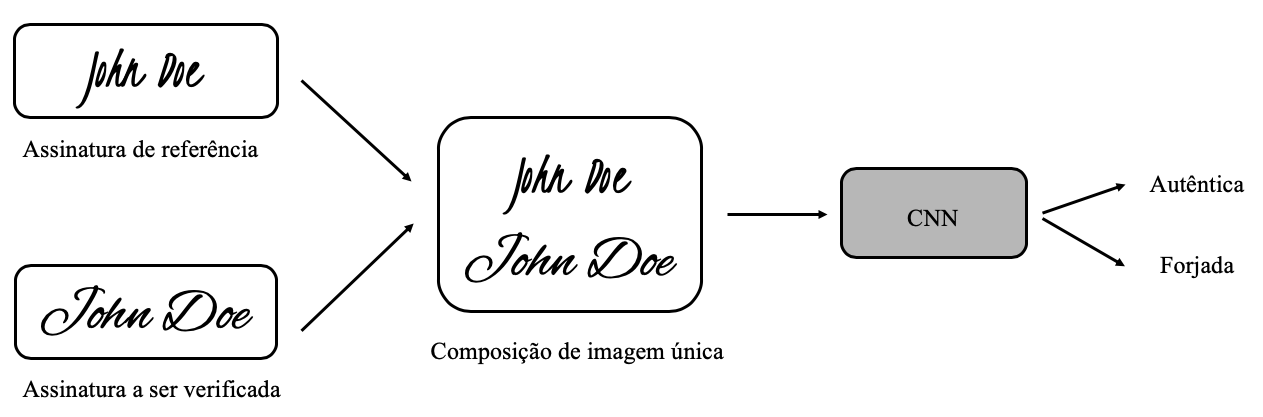
\includegraphics[width=\textwidth]{imgs/esquema-solucao}
\end{figure}

O treinamento e teste das CNNs seguirão o método \emph{holdout} de validação cruzada, em que $70\%$ dos dados serão utilizados no treino e ajuste de parâmetros, enquanto $20\%$ dos dados serão aproveitados para o processo de teste das redes, com vista a capturar o poder de generalização dos modelos considerados. Os $10\%$ de dados restantes, serão utilizados para a validação dos modelos durante o processo de treinamento \cite{brink}.

Os modelos propostos serão avaliados perante as métricas de desempenho de \emph{Acurácia} e \emph{F-score}. A acurácia indica a proporção de predições corretas inferidas pelos modelos. O \emph{F-score}, por sua vez, é calculado pela média harmônica da precisão e da revocação, que assumirá valores diferentes dependendo do balanceamento do conjunto de dados apresentando ao modelo.

Para um \emph{dataset} balanceado, os cálculos da precisão e revocação serão realizados através da técnica de \emph{micro-average}, enquanto para um \emph{dataset} desbalanceado, esses valores serão determinados através do \emph{macro-average}. Nas equações \ref{eq:precision} e \ref{eq:recall} estão demonstrados os valores de precisão ($P$) e revocação ($R$) considerando um problema com duas classes diferentes. Os valores de $TP_n$, $FP_n$ e $FN_n$ são respectivamente os valores de verdadeiros positivos, falsos positivos e falsos negativos aferidos para a classe $n$.

\begin{equation}
\label{eq:precision}
P = \left\{
\begin{array}{lr}
  \frac{TP_1 + TP_2}{TP_1 + FP_1 + TP_2 + FP_2}, & \text{se \emph{micro-average}}\\
  \\
  \frac{P_1 + P_2}{2}, & \text{se \emph{macro-average}}.
\end{array}
\right.
\end{equation}

\begin{equation}
\label{eq:recall}
R = \left\{
\begin{array}{lr}
  \frac{TP_1 + TP_2}{TP_1 + FN_1 + TP_2 + FN_2}, & \text{se \emph{micro-average}}\\
  \\
  \frac{R_1 + R_2}{2}, & \text{se \emph{macro-average}}.
\end{array}
\right.
\end{equation}


\subsection{Visão Geral do Conjunto de Dados}
% estatisticas calculadas lá no notebook
Para a obtenção de um modelo inteligente capaz de verificar a autenticidade de assinaturas de indivíduos, é necessário, primeiramente, treiná-lo. Para tanto, é necessário um conjunto de exemplos, isto é, uma base de dados  que possua exemplos de assinaturas e seus respectivos rótulos, isto é, quando são forjadas ou genuínas, com vistas a prover características relevantes para o aprendizado.

Para este fim, utilizou-se dois conjuntos de dados originalmente disponibilizados pela
\emph{Signature Verification Competition} realizada na \emph{International Conference on Document Analysis and Recognition} em 2009. Na ocasião da competição, cada um destes conjuntos de dados foi utilizado em uma etapa. Na etapa de treinamento, foi utilizado o conjunto de assinaturas do \emph{Norwegian Information Security laboratory and Donders Centre for Cognition} (NISDCC), composto originalmente de 1.920 assinaturas genuínas e forjadas. Para a etapa seguinte, de validação dos modelos submetidos, foi utilizado o conjunto coletado pelo \emph{Netherlands Forensic Institute} (NFI), composto por 1.953 novas assinaturas genuínas e forjadas \cite{icdar2009}. Considerando que a competição ocorreu há uma década, as bases de dados utilizadas na época são atualmente mantidas pela \emph{International Association for Pattern Recognition} (IAPR) e contam com um número de 1.898 assinaturas do conjunto NISDCC e 1.564 assinaturas do conjunto NFI \cite{iapr-tc11}. Esta versão mais recente é amplamente disponibilizada e, por essa razão, está sendo utilizada no escopo deste trabalho.

Os conjuntos disponibilizados pelo IAPR são compostos por dois tipos de assinaturas, as assinaturas \emph{offline} e as assinaturas \emph{online}. Nas assinaturas \emph{offline}, é considerado apenas o aspecto estático da mesma, ou seja, uma imagem obtida após o processo da assinatura ter sido concluído. Estes dados foram segmentados, inspecionados visualmente e, em seguida, pré-processados para fornecer imagens formatadas em cores, em escala de cinza e binárias com a resolução de $600$ dpi. Os dados das assinaturas \emph{online}, por sua vez, continham informações dinâmicas, que consistiam em arquivos de texto que descreviam os detalhes capturados em vários pontos durante o processo da assinatura, sendo estes as coordenadas $x$ e $y$ da ponta da caneta, a pressão exercida sobre a caneta, o ângulo azimutal e o ângulo de elevação \cite{icdar2009}. Um exemplo de uma assinatura \emph{offline} e a sua respectiva representação \emph{online} com os pontos plotados pode ser encontrada na Figura \ref{fig:sample-signature}.


\begin{figure}[h!]
\centering
\caption{Uma amostra das assinaturas \emph{offline} e \emph{online} do SigComp2009. Fonte: \cite{icdar2009}.}
\label{fig:sample-signature}
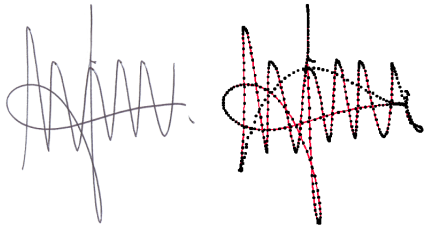
\includegraphics[width=0.5\textwidth]{imgs/sample-signature}
\end{figure}

Nestas bases de dados um certo autor produz várias versões de sua própria assinatura, compondo os exemplos de assinaturas genuínas. Várias pessoas foram convocadas a falsificar esta assinatura, produzindo os exemplos forjados das mesmas. Nestas falsificações utilizou-se a técnica \emph{over-the-shoulder}, na qual o autor forjador tem a oportunidade de visualizar a assinatura genuína antes da falsificação, podendo, inclusive, ter praticado anteriormente diversas vezes. Segundo Blankers et al., este tipo de falsificação costuma ser de difícil detecção \cite{icdar2009}.

Considerando a demanda por equipamentos específicos para obtenção das assinaturas \emph{online} e da pouca existência dos mesmos em cenários práticos, optou-se apenas pela utilização das assinaturas \emph{offline} para a elaboração deste trabalho, com vistas a concentrar os esforços em uma solução que incorpore aspectos de Visão Computacional. Após a exclusão destes exemplos, o quantitativo remanescente de assinaturas e seus tipos (genuína ou forjada) encontram-se disponíveis na Tabela \ref{tab:demonstracao-dataset}.

\begin{table}[h!]
	\centering
	\caption{Quantitativo de indivíduos e assinaturas \emph{offline} por conjunto de dados.}
	\label{tab:demonstracao-dataset}
\resizebox{\textwidth}{!}{
	\begin{tabular}{c C{2cm} C{2cm} C{3.25cm} C{2.5cm} C{2.5cm} C{2.25cm}}
		\toprule
		 \textbf{Conjunto}& \textbf{Autores originais} & \textbf{Autores forjadores} & \textbf{Autores originais com assinaturas forjadas} & \textbf{Assinaturas genuínas}  & \textbf{Assinaturas forjadas} & \textbf{Total de assinaturas} \\
		\midrule
		NISDCC & 12 & 31 & 12 & 60 & 1.838 & 1.898 \\
    NFI & 79 & 33 & 19 & 940 & 624 & 1.564 \\
		\bottomrule
	\end{tabular}}
\end{table}

Conforme pode ser observado, um mesmo autor produziu diferentes versões de sua assinatura. A coluna ``Autores originais'' indica o quantitativo destes indivíduos e a coluna ``Assinaturas genuínas'' indica o total de assinaturas feitas pelos mesmos. No caso do \emph{dataset} NISDCC, em especial, cada autor reproduziu sua própria assinatura $5$ vezes. No NFI não houve uma consistência quantitativa, mas, em média, existem $11$ reproduções da assinatura original pelo autor verdadeiro.

Ainda conforme a Tabela \ref{tab:demonstracao-dataset}, o NISDCC conta com $31$ autores forjadores, os quais produziram versões forjadas de todas as assinaturas originais, mas com um quantitativo de falsificações distintos para cada original, totalizando $1.838$ assinaturas forjadas com a técnica \emph{over-the-shoulder}. No caso do NFI, isto não ocorreu de mesma forma, pois apenas um subconjunto das originais foi alvo de falsificação.

Considerando o total exposto de assinaturas originais e forjadas, tendo sido compreendida a estrutura, organização e exemplos dos \emph{datasets}, partiu-se então para sua preparação com vistas a adequar seu uso para a solução proposta.


\subsection{Preparação do Conjunto de Dados} \label{sec:preparacao}
Sabe-se que algoritmos de AM necessitam de quantidade significantiva de dados, preferencialmente sem muitos ruídos, para serem utilizados de forma a obter um modelo que possua bom desempenho \cite{marsland}. Levando isto em conta e com vistas a adequar os dados disponíveis com a tarefa de aprendizado considerada, uma etapa de pré-processamento fez-se necessárias, cujos passos são descritos a seguir.

Primeiramente foi necessário realizar a adaptação das imagens individuais para as imagens compostas, conforme apresentado anteriormente no esquema da Figura \ref{fig:esquema-solucao}. Para isto, foi feita a combinação de cada assinatura genuína de um autor com suas diferentes versões originais, produzindo uma nova imagem para cada caso a qual associou-se o rótulo de autêntica. Após esta etapa, também foram combinados os exemplos genuínos com suas respectivas versões forjadas, aos quais foi associado o rótulo de forjado. Todas as imagens obtidas dessas combinações serão utilizadas como exemplos para o processo de treinamento, validação e teste do modelo proposto.

O processo de combinação das imagens de cada um dos exemplos foi realizado em três etapas. Na primeira etapa, ambas as imagens foram redimensionadas para um tamanho de $256 \times 256$ \emph{pixels}. Em seguida, as imagens foram concatenadas verticalmente com a intenção de formar uma única imagem de $256 \times 512$ \emph{pixels}. Por fim, a imagem resultante foi redimensionada novamente em um tamanho de $256 \times 256$ \emph{pixels} e transformada para um espaço de cores em escala de cinza, com a intenção de padronizar todas os exemplos.

% Escrever algo sobre como foi atingida a quantidade de exemplos atual?

Ao concluir a etapa anterior, percebeu-se uma desproporção significativa no número de exemplos de cada classe, o que poderia comprometer o processo de aprendizado do modelo. Para contornar este problema, foram então consideradas três abordagens distintas para os exemplos disponíveis:

\begin{enumerate}
	\item \textbf{Abordagem 1}. Considera apenas os exemplos autênticos para os quais há uma versão forjada. Neste cenário, tem-se apenas $15\%$ de exemplos autênticos e $85\%$ de exemplos forjados;
	\item \textbf{Abordagem 2}. Nesta abordagem foi preservado o total de exemplos autênticos da abordagem anterior, mas o excedente de exemplos forjados que causavam um desbalanceamento evidente foram descartados de maneira pseudo-aleatória. Embora contenha menos exemplos, esta abordagem tem um \emph{dataset} balanceado, com mesma proporção para ambas as classes;
	\item \textbf{Abordagem 3}. Visando um melhor aproveitamento das assinaturas originais no \emph{dataset} NFI, considerou o incremento de assinaturas autênticas, ainda que não haja exemplos forjados para mesma. É importante enfatizar que os exemplos forjados desta abordagem são iguais ao da primeira. Obteve-se, então, um \emph{dataset} com mais exemplos e \emph{quasi}-balanceado.
\end{enumerate}

Após a organização dos exemplos conforme as abordagens distintas, realizou-se então a partição \emph{holdout} de validação cruzada, com $70\%$ dos exemplos para treinamento, $10\%$ para validação e $20\%$ para testes. A Tabela \ref{tab:divisao-dados} apresenta a descrição destes dados, suas quantidades e divisões e a Figura \ref{fig:divisao-dados} auxilia na visualização da proporcionalidade nas diferentes abordagens consideradas.

\begin{table}[h!]
	\centering
	\caption{Quantitativo de exemplos por abordagem, classe e finalidade na tarefa de aprendizado considerada.}
	\label{tab:divisao-dados}
\resizebox{\textwidth}{!}{
	\begin{tabular}{c c c c c c c c}
		\toprule
		\textbf{Abordagem} & \textbf{Característica} & \textbf{Tipo de Exemplo} & \textbf{Treino} & \textbf{Validação} & \textbf{Teste} & \textbf{Total} & \textbf{Proporção}\\
		\midrule
		\multirow{2}{*}{1} & \multirow{2}{*}{Dados desbalanceados} & Genuíno & 2.011 & 299 & 618 & 2.928 & $15\%$ \\
    &  & Forjado & 11.649 & 1.648 & 3.237 & 16.534 & $85\%$\\
     \midrule
    \multirow{2}{*}{2} & \multirow{2}{*}{Dados balanceados} & Genuíno & 2.011 & 299 & 618 & 2.928 & $50\%$  \\
    &  & Forjado & 2.024 & 308 & 569 & 2.901 & $50\%$ \\
		 \midrule
		\multirow{2}{*}{3} & \multirow{2}{*}{Dados \emph{quasi}-balanceados} & Genuíno & 8.131 & 1.134 & 2.257  & 11.522 & $41\%$\\
		 & & Forjado & 11.649 & 1.648 & 3.237 & 16.534 & $59\%$\\
		\bottomrule
	\end{tabular}}
\end{table}

\begin{figure}[h!]
	\centering
	\caption{Representação gráfica da proporção dos exemplos por abordagem, classe e finalidade na tarefa de aprendizado considerada.}
	\subfloat[Abordagem 1\label{subfig:approach1}]{%
	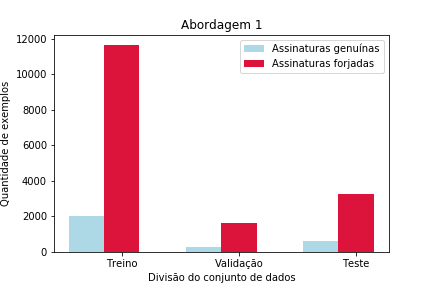
\includegraphics[width=0.5\textwidth]{imgs/approach1}
	}
	\subfloat[Abordagem 2\label{subfig:approach2}]{%
	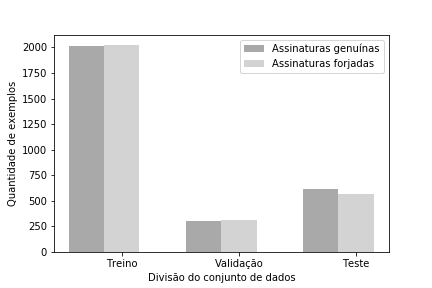
\includegraphics[width=0.5\textwidth]{imgs/approach2}
	}
	\hfill
	\subfloat[Abordagem 3\label{subfig:approach3}]{%
	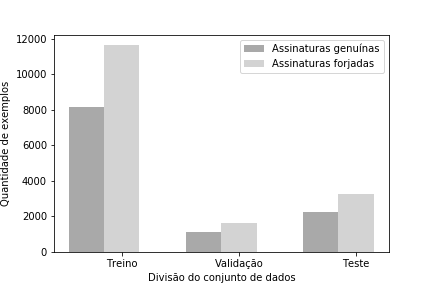
\includegraphics[width=0.5\textwidth]{imgs/approach3}
	}
	\label{fig:divisao-dados}
\end{figure}

Ao serem fornecidas para treinamento pelas CNNs, todas os \emph{pixels} das imagens serão normalizados por meio de uma divisão por $255$, passando a residirem no intervalo $[0,1]$. Esta normalização é realizada em virtude das redes neurais que, em geral, aprendem mais eficientemente nestas condições \cite{chollet}.


\subsection{Modelos, Parâmetros e Hiperparâmetros de CNNs Considerados}
%!TEX root = ../../main.tex

Como visto anteriormente, propor arquiteturas eficientes de CNNs que obtenham bom desempenho em determinada tarefa de aprendizado é considerada uma atividade difícil. Para contornar esta dificuldade, para o problema considerado neste trabalho, escolheu-se então utilizar topologias canônicas de CNNs, que obtiveram bons desempenhos reportados pela literatura, mas promovendo ajustes em seus parâmetros e hiperparâmetros com a finalidade de buscar melhorias  no desempenho para a tarefa de aprendizado aqui definida. Dentre estas arquiteturas canônicas, as selecionadas para o escopo deste trabalho encontram-se descritas a seguir:

\begin{itemize}
	\item \textbf{LeNet}. Desenvolvida por LeCun em 1989, a arquitetura LeNet foi uns dos primeiros exemplos da aplicação de CNNs, tendo sido utilizada para a detecção de dígitos manuscritos utilizando o dataset MNIST \cite{lecun}. Possui um total de 7 camadas e aproximadamente $7$ milhões de parâmetros treináveis;
	\item \textbf{AlexNet}. Em 2012, a arquitetura AlexNet foi a primeira CNN a vencer o desafio ILSVRC da ImageNet, com uma boa margem de diferença dos outros modelos submetidos à competição. Para o seu treinamento com o conjunto de dados ImageNet, foram utilizadas duas GPUs de 3 GB de memória cada, que foram capazes de armazenar o processamento de aproximadamente 62 milhões de parâmetros \cite{alexnet,khan};
	\item \textbf{SqueezeNet}. Foi desenvolvida em 2016 através de uma parceria entre os cientistas da DeepScale, University of California, Berkeley e Stanford University. A idéia foi criar uma arquitetura com o nível de acurácia da AlexNet com $50$ vezes menos parâmetros e com um tamanho $0.5$ MB menor, permitindo uma maior eficiência no treinamento em sistemas distribuídos, menor sobrecarga na exportação de modelos através da rede e sua capacidade de ajustar-se a sistemas com pouca memória \cite{squeezenet};
	\item \textbf{MobileNet}. Constituída por um conjunto de dois hiperparâmetros, esta arquitetura possui menor latência e um tamanho menor comparada às outras arquiteturas existentes, possuindo os requisitos que facilitam a sua implementação em aplicações para dispositivos móveis e embarcados \cite{mobilenet}. No \emph{framework} \texttt{keras}, utilizado nas atividades realizadas neste trabalho, esta arquitetura possui uma profundidade de $88$ camadas, $4.253.864$ parâmetros e um tamanho de 17 MB \cite{keras};
	\item \textbf{ShuffleNet}. Esta arquitetura se destaca pela sua composição de convoluções em grupo, na qual diversas convoluções são efetuadas paralelamente tomando porções dos canais de entrada, diminuindo de maneira eficiente o custo computacional. Posteriormente, os canais de saída da convolução em grupo são mesclados aleatoriamente através do processo chamado de \emph{channel shuffle} \cite{shufflenet};
	\item \textbf{VGG-16}. Esta CNN, que consiste em 16 camadas convolucionais, possui arquitetura uniforme e é comumente muito utilizada na extração de características em imagens. Possuindo mais de 138 milhões de parâmetros e uma profundidade de 23 camadas, esta arquitetura possui um tamanho total de 528 MB no módulo \texttt{applications} do \texttt{keras} \cite{vgg16, keras};
	\item \textbf{Inception}. Também chamada de GoogleNet, esta arquitetura é conhecida por ser a primeira a se desviar da forma padrão de simplesmente sequenciar camadas convolucionais e de \emph{pooling}, criando os chamados blocos \emph{Inception}. A sua versão InceptionV3 presente na biblioteca \texttt{keras} possui um total de $23.851.784$ parâmetros e um tamanho de 92 MB \cite{inception, keras}.
\end{itemize}

Em relação aos modelos adotados, considerou-se uma modificação na arquitetura geral apenas para compatibilizá-los ao problema considerado, que consiste em uma tarefa de aprendizado binária. Esta alteração diz respeito à camada de saída que consiste em apenas um neurônio com função de ativação sigmoidal, a qual retornará a probabilidade de pertencimento à cada classe na tarefa considerada.

Uma vez definidas as arquiteturas que serão utilizadas, define-se, em consequência, os parâmetros a serem adotados, que estão relacionados aos pesos destas redes, os quais serão obtidos via treinamento segundo \emph{backpropagation}. Os hiperparâmetros, por sua vez, dizem respeito  ao ajuste em nível de arquitetura das CNNs \cite{chollet}. No escopo deste trabalho, considerou-se variações nos valores dos seguintes hiperparâmetros: otimizador para o cálculo do gradiente descendente, função de ativação das camadas intermediárias e \emph{patience}, em que este último corresponde a um valor para interromper o treinamento da rede mediante \emph{early stopping} a fim de evitar \emph{overfitting}. Os valores adotados encontram-se dispostos na Tabela \ref{tab:parametros}.

\begin{table}[h!]
	\centering
	\caption{Valores dos hiperparâmetros selecionados para a elaboração dos modelos.}
	\label{tab:parametros}
	\begin{tabular}{c c C{3cm} C{3cm}}
		\toprule
		 \textbf{Épocas} & \textbf{\emph{Patience}} & \textbf{Otimizador} & \textbf{Função de ativação}  \\
		\midrule
		200 & 5, 10 e 15 & SGD, Adam e RMSprop & ReLU, ELU, SELU e Leaky ReLU \\
		\bottomrule
	\end{tabular}
\end{table}

De maneira mais detalhada, com a adoção de \emph{early stopping}, passou-se a monitorar uma métrica de desempenho durante o treinamento da rede, podendo esta ser a perda no conjunto de treinamento ou a acurácia no conjunto de validação, por exemplo. Com o uso de um valor de \emph{patience}, sempre que a métrica monitorada não melhorava durante o treinamento, decrementou-se uma unidade. O treinamento foi finalizado, então, quando este valor tornou-se igual a zero \cite{chollet}. Os valores adotados para \emph{patience}, no escopo deste trabalho, foram obtidos de maneira empírica em testes preliminares.

Um otimizador tem como objetivo aumentar o desempenho de um modelo de AM, ajustando os seus parâmetros com vistas a diminuir o erro encontrado na etapa de treinamento de tal modelo. Para o escopo deste trabalho, foram utilizados três otimizadores diferentes, sendo eles, o SGD (\emph{stochastic gradient descent}), RMSprop e o Adam (do inglês \emph{adaptive moment estimation}).

No SGD, a superfície de erro é estimada apenas com respeito a um único exemplo, tornando essa superfície dinâmica. Como resultado, descer nessa superfície melhora significativamente a habilidadede de navegar por regiões planas. O RMSprop, por sua vez, utiliza-se do valor do gradiente da função de custo e da sua raiz média quadrática para atualizar os pesos da CNN. O RMSProp tem mostrado ser um eficiente otimizador para redes neurais profundas e é a escolha principal para muitos praticantes experientes em criação de modelos de DL. E por fim, o otimizador Adam, é um algoritmo que pode ser considerado como a combinação do RMSprop com o \emph{momentum}, que possui base em estimativas adaptativas de momentos de menor ordem. É computacionalmente eficiente e demanda poucos requisitos de memória, sendo adequado para para problemas que possuem grande quantidade dados ou parâmetros \cite{buduma, rmsprop, adam}.

As funções de ativação ReLU e as suas variações \emph{Leaky} ReLU, ELU (\emph{Exponential Linear Unit}) e SELU (\emph{Scaled Exponential Linear Unit}) foram escolhidas para estarem presentes nos neurônios das camadas internas das CNNs por auxiliarem na captura de relações não-lineares. Embora a função ReLU seja amplamente adotada, optou-se também por utilizar suas variações, pois para esta pode incorrer o chamado ``\emph{dying ReLU problem}'', que acontece quando os neurônios com esta função de ativação tornam-se inativos e produzem apenas a saída zero para toda entrada \cite{reluDying}.  Desta maneira, a sua variante \emph{Leaky ReLU} mostrou ser uma boa escolha, pois possui um parâmetro adicional $\alpha$, chamado de vazamento, que faz com que o gradiente seja pequeno, mas nunca nulo. A função ELU também é uma boa alternativa à ReLU pois diminui a mudança do \emph{bias} ao pressionar a ativação média para zero. A SELU, por sua vez, possui uma auto-normalização, fazendo com que a aprendizagem seja altamente robusta e permitindo treinar redes com muitas camadas \cite{relu}. Na Figura \ref{fig:relu-variants} encontram-se os gráficos das variações da função ReLU.

\begin{figure}[h!]
	\centering
	\caption{Funções de ativação variantes da função ReLU.}\label{fig:relu-variants}
	\subfloat[\emph{Leaky} ReLu\label{subfig:lrelu}]{%
	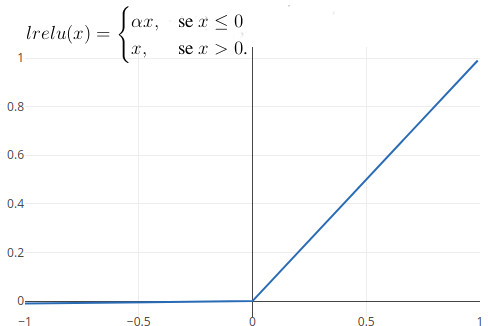
\includegraphics[width=0.5\textwidth]{imgs/lrelu}
	}
	\hfill
	\subfloat[ELU\label{subfig:elu}]{%
	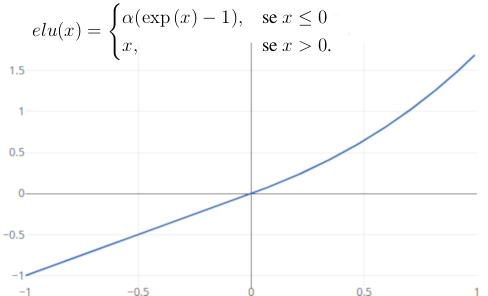
\includegraphics[width=0.5\textwidth]{imgs/elu}
	}
	\subfloat[SELU\label{subfig:selu}]{%
	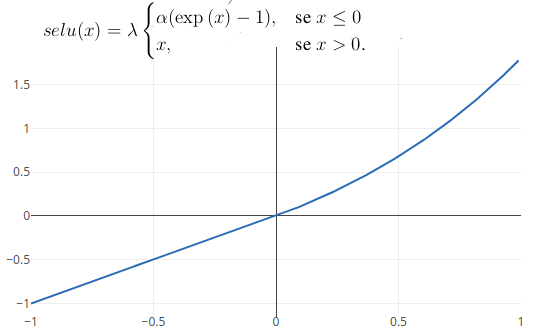
\includegraphics[width=0.5\textwidth]{imgs/selu}
	}
\end{figure}

% \begin{equation}
%     lrelu(x)=
% \begin{cases}
%     \alpha x , & \text{se } x \leq 0\\
%     x,              & \text{se } x > 0\text{.}
% \end{cases}
% \end{equation}
%
% \begin{equation}
%     elu(x)=
% \begin{cases}
%     \alpha (\exp{(x)} - 1) , & \text{se } x \leq 0\\
%     x,              & \text{se } x > 0\text{.}
% \end{cases}
% \end{equation}
%
% \begin{equation}
%     selu(x)= \lambda
% \begin{cases}
%     \alpha (\exp{(x)} - 1) , & \text{se } x \leq 0\\
%     x,              & \text{se } x > 0\text{.}
% \end{cases}
% \end{equation}

Sempre que os recursos computacionais e de tempo para o treinamento viabilizaram repetições, foram consideradas todas as variações possíveis dos hiperparâmetros descritos na Tabela \ref{tab:parametros}. Nas demais situações foram consideradas escolhas de hiperparâmetros com melhor desempenho nos cenários que já tiverem sido executados. % Ad hoc?

